\documentclass[fullapage,12pt]{article}
\usepackage{fancybox}
\usepackage{graphicx}
\usepackage{amssymb}
\usepackage{amsmath}
\usepackage{epsfig}
\usepackage{color}
\usepackage{multicol}
\usepackage{hhline}
\usepackage{xspace,epic,eepic,graphicx}
\usepackage{latexsym}
\usepackage{enumerate}

\newcommand{\mc}[1]{\mathcal{ #1}}
\newcommand{\e}[1]{\emph{#1}}
\newcommand{\ignore}[1]{}
\newcommand{\boxtheorem}{\hfill $\Box$\\}
\newcommand{\nit}[1]{{\it #1}}



\begin{document}
\thispagestyle{empty}

\vspace*{-3.5cm}
\begin{center} \bf \large COMP 3400~ Computational Logic and Automated Reasoning\\ Winter 2017~~ Assignment 2
\end{center}

{\small \noindent {\bf Instructions:}
\begin{enumerate}
\item {\bf \Large For your solution use the template file that was posted on the course news, and follow the instructions in it.}

In particular: (a) Include at the top of the first page: full name, student number, and email address.
(b) {\bf Assignments have to be created with Latex, and submitted in pdf format, as a single file}. (c) Every problem solution MUST include
the problem statement, even if the assignment does not (sometimes the assignments will refer to slides presented in class). The source file for this assignment is provided.

Latex has to be used as such, not as you would use a text editor, such as Notepad. In particular,  formulas have to be written using Latex's mathematical
features, and then compiled.

\item Assignments are individual, no groups.
\item  %Use the same format as this document (the Latex source is provided with the pdf).
Submit by email to the instructor, with ``Assignment "Number", CompLog" in the subject. {\bf Include your last name in the file name!} For example,
in the subject: \ ``Assig. 2 CompLog". The file name: \ ``bertossi-2.pdf".

{\bf Only a single pdf file will be accepted as submission (nothing other than a pdf file will be accepted). No tar or zip files (or anything like that), please. Keep your Latex source files in case you are requested to show them.}

\item Explain your solution very carefully, but still be succinct with your answers. No unnecessary verbose arguments, please. Go to the point.

Make explicit all your assumptions.

\item {\bf Not following the instructions above or the solution template file will make you lose points.}
\end{enumerate}}


\noindent 1. \ Prove using {\bf PROPOSITIONAL} logic and Prover9 that the map (cf. Fig. \ref{fig:map}) that includes Chile, Peru,
Argentina and Bolivia cannot be painted with two colors if adjacent countries must have different colors.
To simplify, assume that the colors are blue and green. \ More precisely:
\begin{enumerate}[(a)]
\item  Before doing anything with Prover9 (and independently from its input file), write the knowledge basis in propositional logic. 
\item Describe the methodology you will use (all this before going into Prover9). The methodology should be general enough to work in essence with any map and number of colors.
Discuss to what extent your methodology is general and declarative (as opposed to a hack for this very particular map). 

\item Do the proof with Prover9, including the input and output text files for/from Prover9 as an appendix (better use the verbatim environment in Latex).
It has to contain all the formulas, the knowledge base created by Prover9, and the final clean proof.


%\vspace*{-3cm}
\begin{figure}[h]
\begin{center}
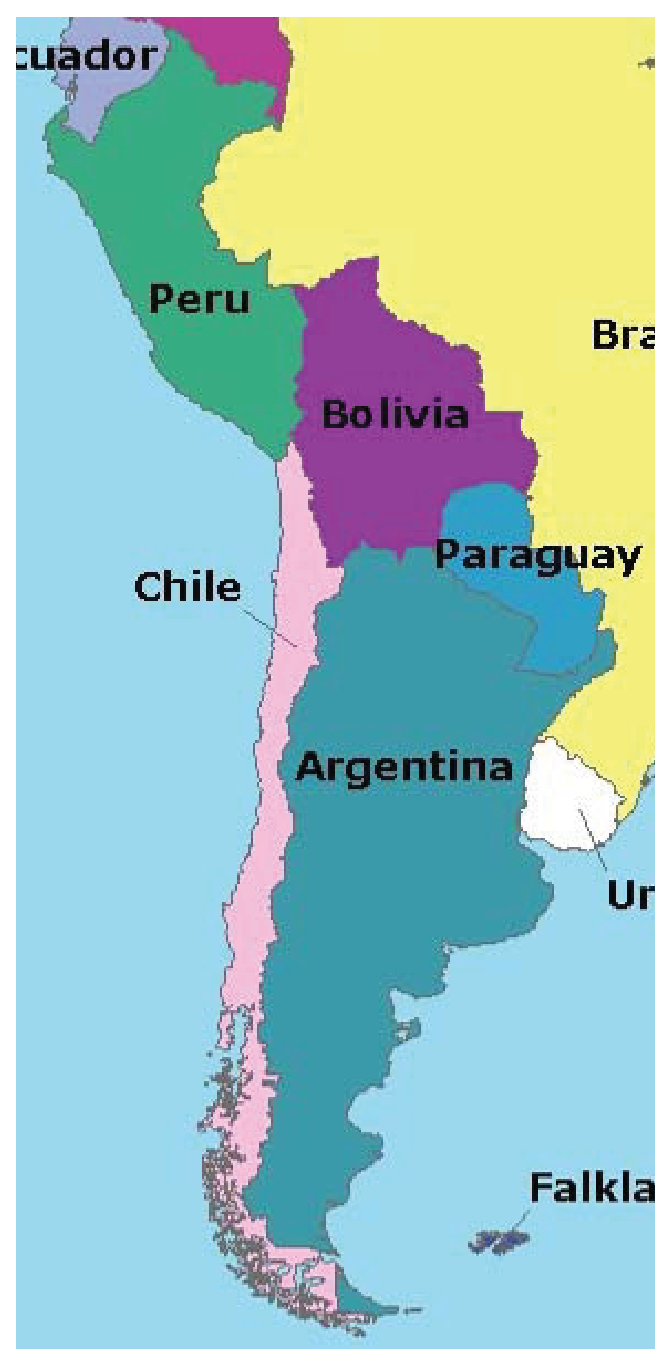
\epsfig{file=mapSA.eps,width=4cm}
\caption{Part of South America}\label{fig:map}
\end{center}
\end{figure}

\end{enumerate}

\noindent
2. \ Do the same as in the previous problem, and with the same requests, with {\bf PREDICATE} logic. For that you can use predicates for ``being neighbors" and ``having a color", 
and symbolic constants for the four countries and the two colors.\\

\noindent {\bf Deadline: \ Feb. 17, at 23:55}




\end{document}
